\section{Slučajevi upotrebe}
\label{subsec:podnaslov2}
\subsection {Podnošenje zahteva za prijavu}
Proces registracije korisnika u auto školi započinje popunjavanjem online formulara, gde kandidat unosi svoje lične podatke. Administrativni radnik treba da proveri da kadnidat ispunjava potrebne uslove za upis i formira neophodnu dokumentaciju za kandidata. Nakon toga informacije prosleđuje administratoru sistema, koji unosi novog korisnika u bazu i prosleđuje radniku ID za trenutnog korisnika. Kada je kandidat prijavljen u auto školu, dobija imejl sa potvrdom o registraciji i svoj ID, pa se može ulogovati na svoj nalog. 

\subsubsection{Podnošenje prijave}
\label{subsubsec:prijava}
\begin{itemize}
  \item \textbf{Kratak opis}: Da bi kandidat započeo obuku u auto školi, prvo mora da podnese prijavu za upis. Popunjava online formular, gde unosi svoje lične podatke, koji se nakon potvrde šalju administrativnom radniku. Radnik formira dokumentaciju za kandidata i prosleđuje ih administratoru sistema, koji unosi informacije o kandidatu u sistem.
  \item \textbf{Učesnici}: 
    \begin{itemize} 
      \item Kandidat
      \item Administrativni radnik
      \item Administrator sistema
    \end{itemize} 
  \item \textbf{Preduslovi}:
    \begin{itemize}
    \item Kandidat mora posedovati važeću ličnu kartu.
    \item Kandidat mora uplatiti prvu ratu.
    \end{itemize}
  \item \textbf{Postuslovi}:
      \begin{itemize}
      \item Kandidat ispunjava uslove za prijavu.
      \end{itemize}
  \item \textbf{Osnovni tok}:
      \begin{enumerate}
        \item Kandidat otvara online formu za prijavu u auto školu.
        \item Sistem prikazuje formu kandidatu.
        \item Kandidat popunjava formu, unoseći sve potrebne informacije.
        \item Kanidat šalje unete podatke klikom na dugme “Pošalji”.
        \item Sistem validira unos podataka.
        \item Sistem čuva podatke.
        \item Sistem prosleđuje podatke administrativnom radniku.
        \item Аdministrativni radnik proverava da li kanidat ispunjava uslove za upis.
        \item Administrativni radnik formira dokumentaciju za kandidata.
        \item Administrativni radnik prosleđuje podatke o kandidatu administratoru sistema.
      \end{enumerate}

  \item \textbf{Alternativni tokovi}:
      \begin{itemize}
        \item A1. \textbf{Kandidat ne ispunjava uslove za upis.}
        Ukoliko je u koraku 4 administrativni radnik uočio da kandidat ne ispunjava uslove za prijavu i kontaktira ga kako bi ga obavestio o tome i ispravio podatke ukoliko je moguće. Proces se nastavlja u 1. koraku osnovnog toka.
      \end{itemize}

  \item \textbf{Dodatne informacije}:\newline
  Potrebni podaci za prijavu su ime, prezime, JMBG, broj telefona, imejl adresa i potvrda o uplati prve rate.
\end{itemize}

\begin{figure}[H]
  \begin{center}
      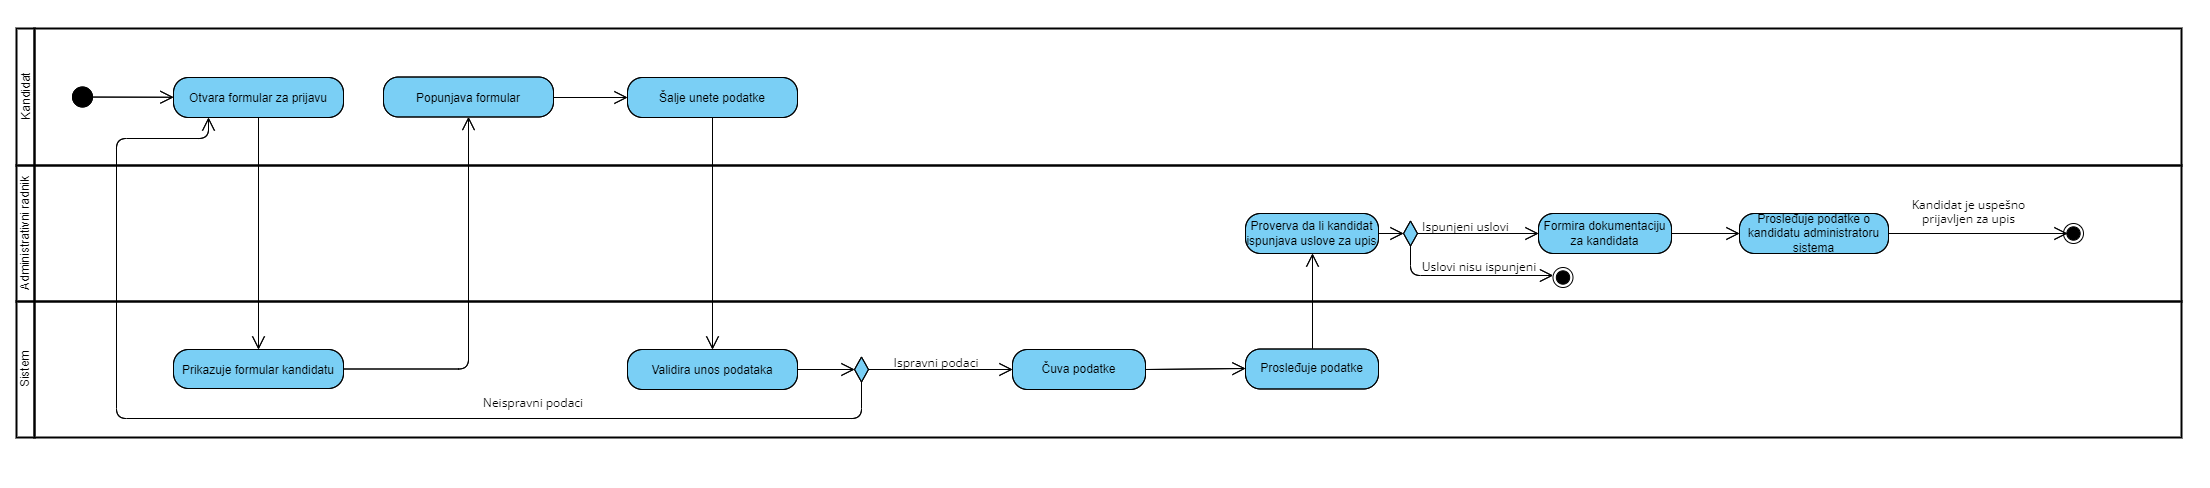
\includegraphics[width=140mm, height=70mm]{Diagrams/dijagram_aktivnosti_podnosenje_prijave.png}
  \end{center}
  \caption {Dijagram aktivnosti - Podnošenje prijave}
  \label{activity_podnosenje_prijave}

\end{figure}





\subsubsection{Registracija kandidata}
\label{subsubsec:registracija}
\begin{itemize}
  \item \textbf{Kratak opis}: Da bi kandidat mogao da se uloguje na svoj nalog i vidi svoje podatke, nepohodno je da dobije potvrdu da je upisan u auto školu, kao i nepohodan ID za logovanje.
  \item \textbf{Učesnici}:
  \begin{itemize}
    \item Kandidat
    \item Administrator sistema
    \item Administrativni radnik.
  \item \textbf{Preduslovi}:
    \begin{itemize}
    \item  Kandidat je popunio online prijavu.
    \item  Kandidat ispunjava uslove za upis.
    \end{itemize}
  \item \textbf{Postuslovi}:
      \begin{itemize}
      \item Kandidat je evidentiran u sistemu.
      \item Kandidat može da se prijavi na sistem.
      \end{itemize}
  \item \textbf{Osnovni tok}:
      \begin{enumerate}
        \item Administrator sistema prima informacije o novom kadnidatu.
        \item Administrator sistema unosi novog korisnika u bazu podataka.
        \item Sistem čuva unete podatke.
        \item Sistem šalje mejl novom kandidatu sa njegovim ID-jem.
        \item Sistem šalje mejl administrativnom radniku da je uspešno dodao novog kanidata.
        \item Administrativni radnik poziva kadnidata telefonom i proverava da li je dobio mejl sa svim potrebnim informacijama za prijavljivanje.
        \item Administrativni radnik ažurira spisak prijavljenih kandidata dodavanjem novog kadnidata.    
      \end{enumerate}

  \item \textbf{Alternativni tokovi}:
      \begin{itemize}
        \item A1. \textbf{Kandidat nije dobio mejl sa ID-jem i šifrom za pristupanje svom nalogu.}
        Ukoliko u koraku 4 kandidat nije dobio mejl, administrator sistema zahteva od sistema da ponovo pošalje mejl. Proces se nastavlja u koraku 4. osnovnog toka.
        \item A2. \textbf{Administrativni radnik ne može da kontaktira kadnidata.}
        Ukoliko u koraku 6 administrativni radnik ne može da stupi u kontakt sa kandidatom, trenutno stanje sistema se pamti i prekida se slučaj upotrebe na neko vreme. Naredni dan se slučaj upotrebe nastavlja ponovnim pozivom kandidata odnosno proces se nastavlja od 6. koraka osnovnog toka.
      \end{itemize}
\end{itemize}

\subsubsection{Raspoređivanje kandidata u grupu}
\label{subsubsec:grupe}
\begin{itemize}
  \item \textbf{Kratak opis}: Da bi kandidat bio raspoređen u grupu neophodno je da odabere neku od ponuđenih grupa, nakon logovanja na svoj nalog. 
  \item \textbf{Učesnici}: 
    \begin{itemize}
    \item  Kandidat - korisnik sistema koji bira grupu za teorijsku nastavu.
    \end{itemize}
  \item \textbf{Preduslovi}:
    \begin{itemize}
    \item Kandidat je dobio svoj ID i lozinku na mejl.
    \item Kandidat ima pristup internetu.
    \item Sistem je u funkciji.
    \end{itemize}
  \item \textbf{Postuslovi}:
      \begin{itemize}
      \item Kandidat je raspoređen u neku grupu.
      \end{itemize}
  
     
  \item \textbf{Osnovni tok}: 
      \begin{enumerate}
        \item Kandidat se prijavljuje na nalog.
        \item Kandidat klikom na dugme “Grupe” bira neku od ponuđenih grupa.
        \item Sistem šalje mejl kandidatu da je uspešno raspoređen u grupu i raspored održavanja časova.
        \item Kandidat dobija mejl sa podacima o grupi i rasporedu nastave.
      \end{enumerate}

  \item \textbf{Alternativni tokovi}:
      \begin{itemize}
        \item A1. \textbf{Neuspešno prijavljivanje.}
        Kandidat je pogrešio ID ili šifru u koraku 1, pa je nepohodno da proveri ispravnost podataka i da ih ponovo unese. Proces se nastvalja od koraka 1. osnovnog toka.
        \item A2. \textbf{Kandidat nije dobio mejl o raspoređivanju po grupama.}
        Kandidat nije raspoređen u željenu grupu, jer nije dobio mejl sa potvrdom u koraku 4, možda jer je vreme za prijavu isteklo (neko drugi je odabrao preostalo mesto). Proces se nastavlja od koraka 1. osnovnog toka.
      \end{itemize}


  \item \textbf{Specijalni zahtevi}:\newline
      Podaci koji su potrebni kako bi kandidat mogao da se uloguje su ID i lozinka u bazi.
\end{itemize}

  

\begin{figure}[H]
  \begin{center}
      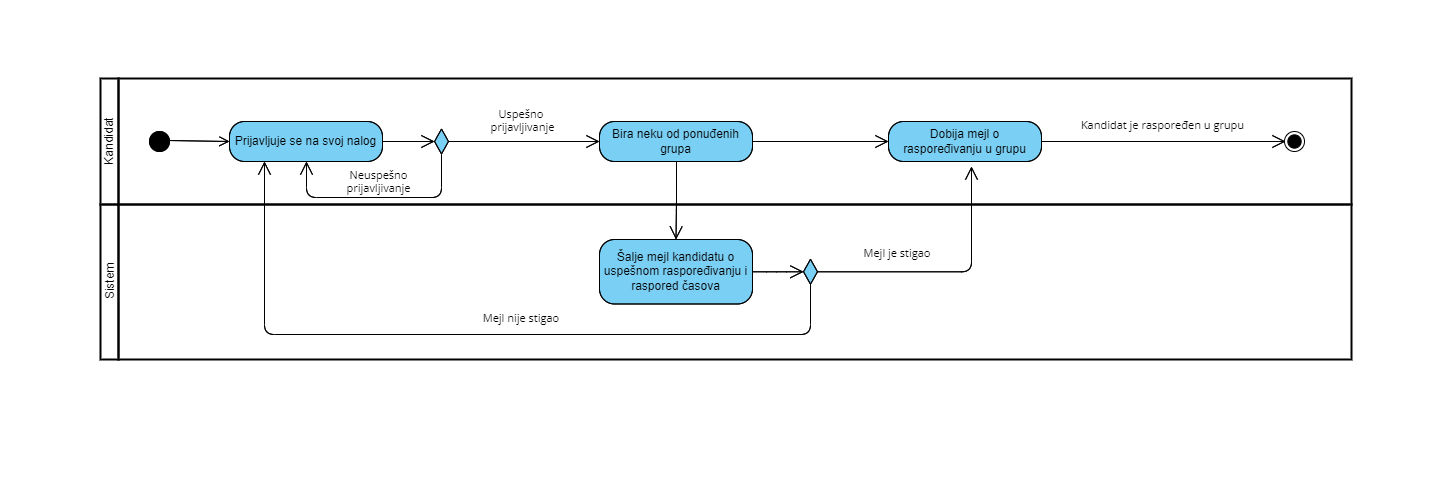
\includegraphics[width=140mm, height=70mm]{Diagrams/dijagram_aktivnosti_grupe.png}
  \end{center}
  \caption {Dijagram aktivnosti - Raspoređivanje kandidata u grupu}
  \label{activity_grupe}

\end{figure}